\documentclass{beamer}
\usepackage{amssymb}
\setbeamertemplate{navigation symbols}{}
\setbeamertemplate{footline}[page number]
\usepackage{amsmath}
\usepackage{amsrefs}
\usepackage{graphicx}
\usepackage{bookman}
\usepackage{url}
\usepackage{amsthm}
\usepackage{verbatim}
\usepackage{xcolor}
\bibliographystyle{amsmath}
\usetheme{Madrid}
\usecolortheme{dolphin}
\useoutertheme[footline=authortitle]{miniframes}

%\newtheorem{theorem}{Theorem}[section]
%\newtheorem{corollary}[theorem]{Corollary}

\title[]{Right Whale Recognition}
\author[]{Tyler Allen\\ \footnotesize Clemson University}
\date{\vspace{-10ex}}
\begin{document}

%\setbeamercolor{title}
\begin{frame}
\begin{center}
\maketitle
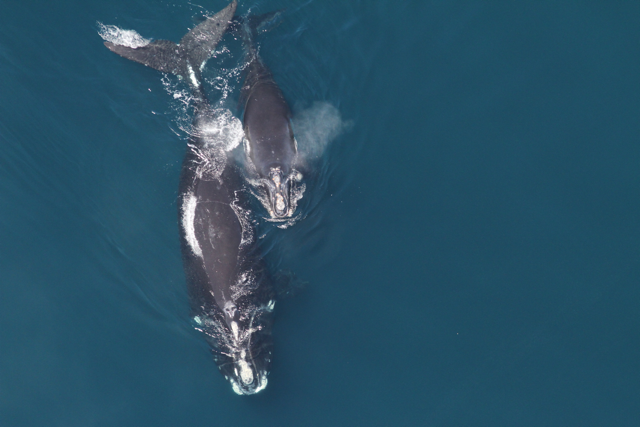
\includegraphics[scale=.20]{title.png}
\end{center}
\end{frame}

\begin{frame}{Motivation}
\begin{itemize}
\item Project from kaggle.com
\item Less than 500 right whales remaining
\item Biologists identify whales by hand
\item Only a few researchers can do this
\end{itemize}
\end{frame}


\begin{frame}{Goals}
\begin{itemize}
\item Data set is photographs of right whales
\item Problem 1: Find right whales
\item Problem 2: Match whale to identification number
\end{itemize}
\end{frame}

\begin{frame}{Strategy Overview}
\begin{itemize}
\item Use photo recognition to find whales
\item Crop found whales from photos
\item Use various algorithms to identify
\end{itemize}
\end{frame}

\section{Recognition}
\subsection{Recognition}
\begin{frame}{Data Example}
\begin{figure}
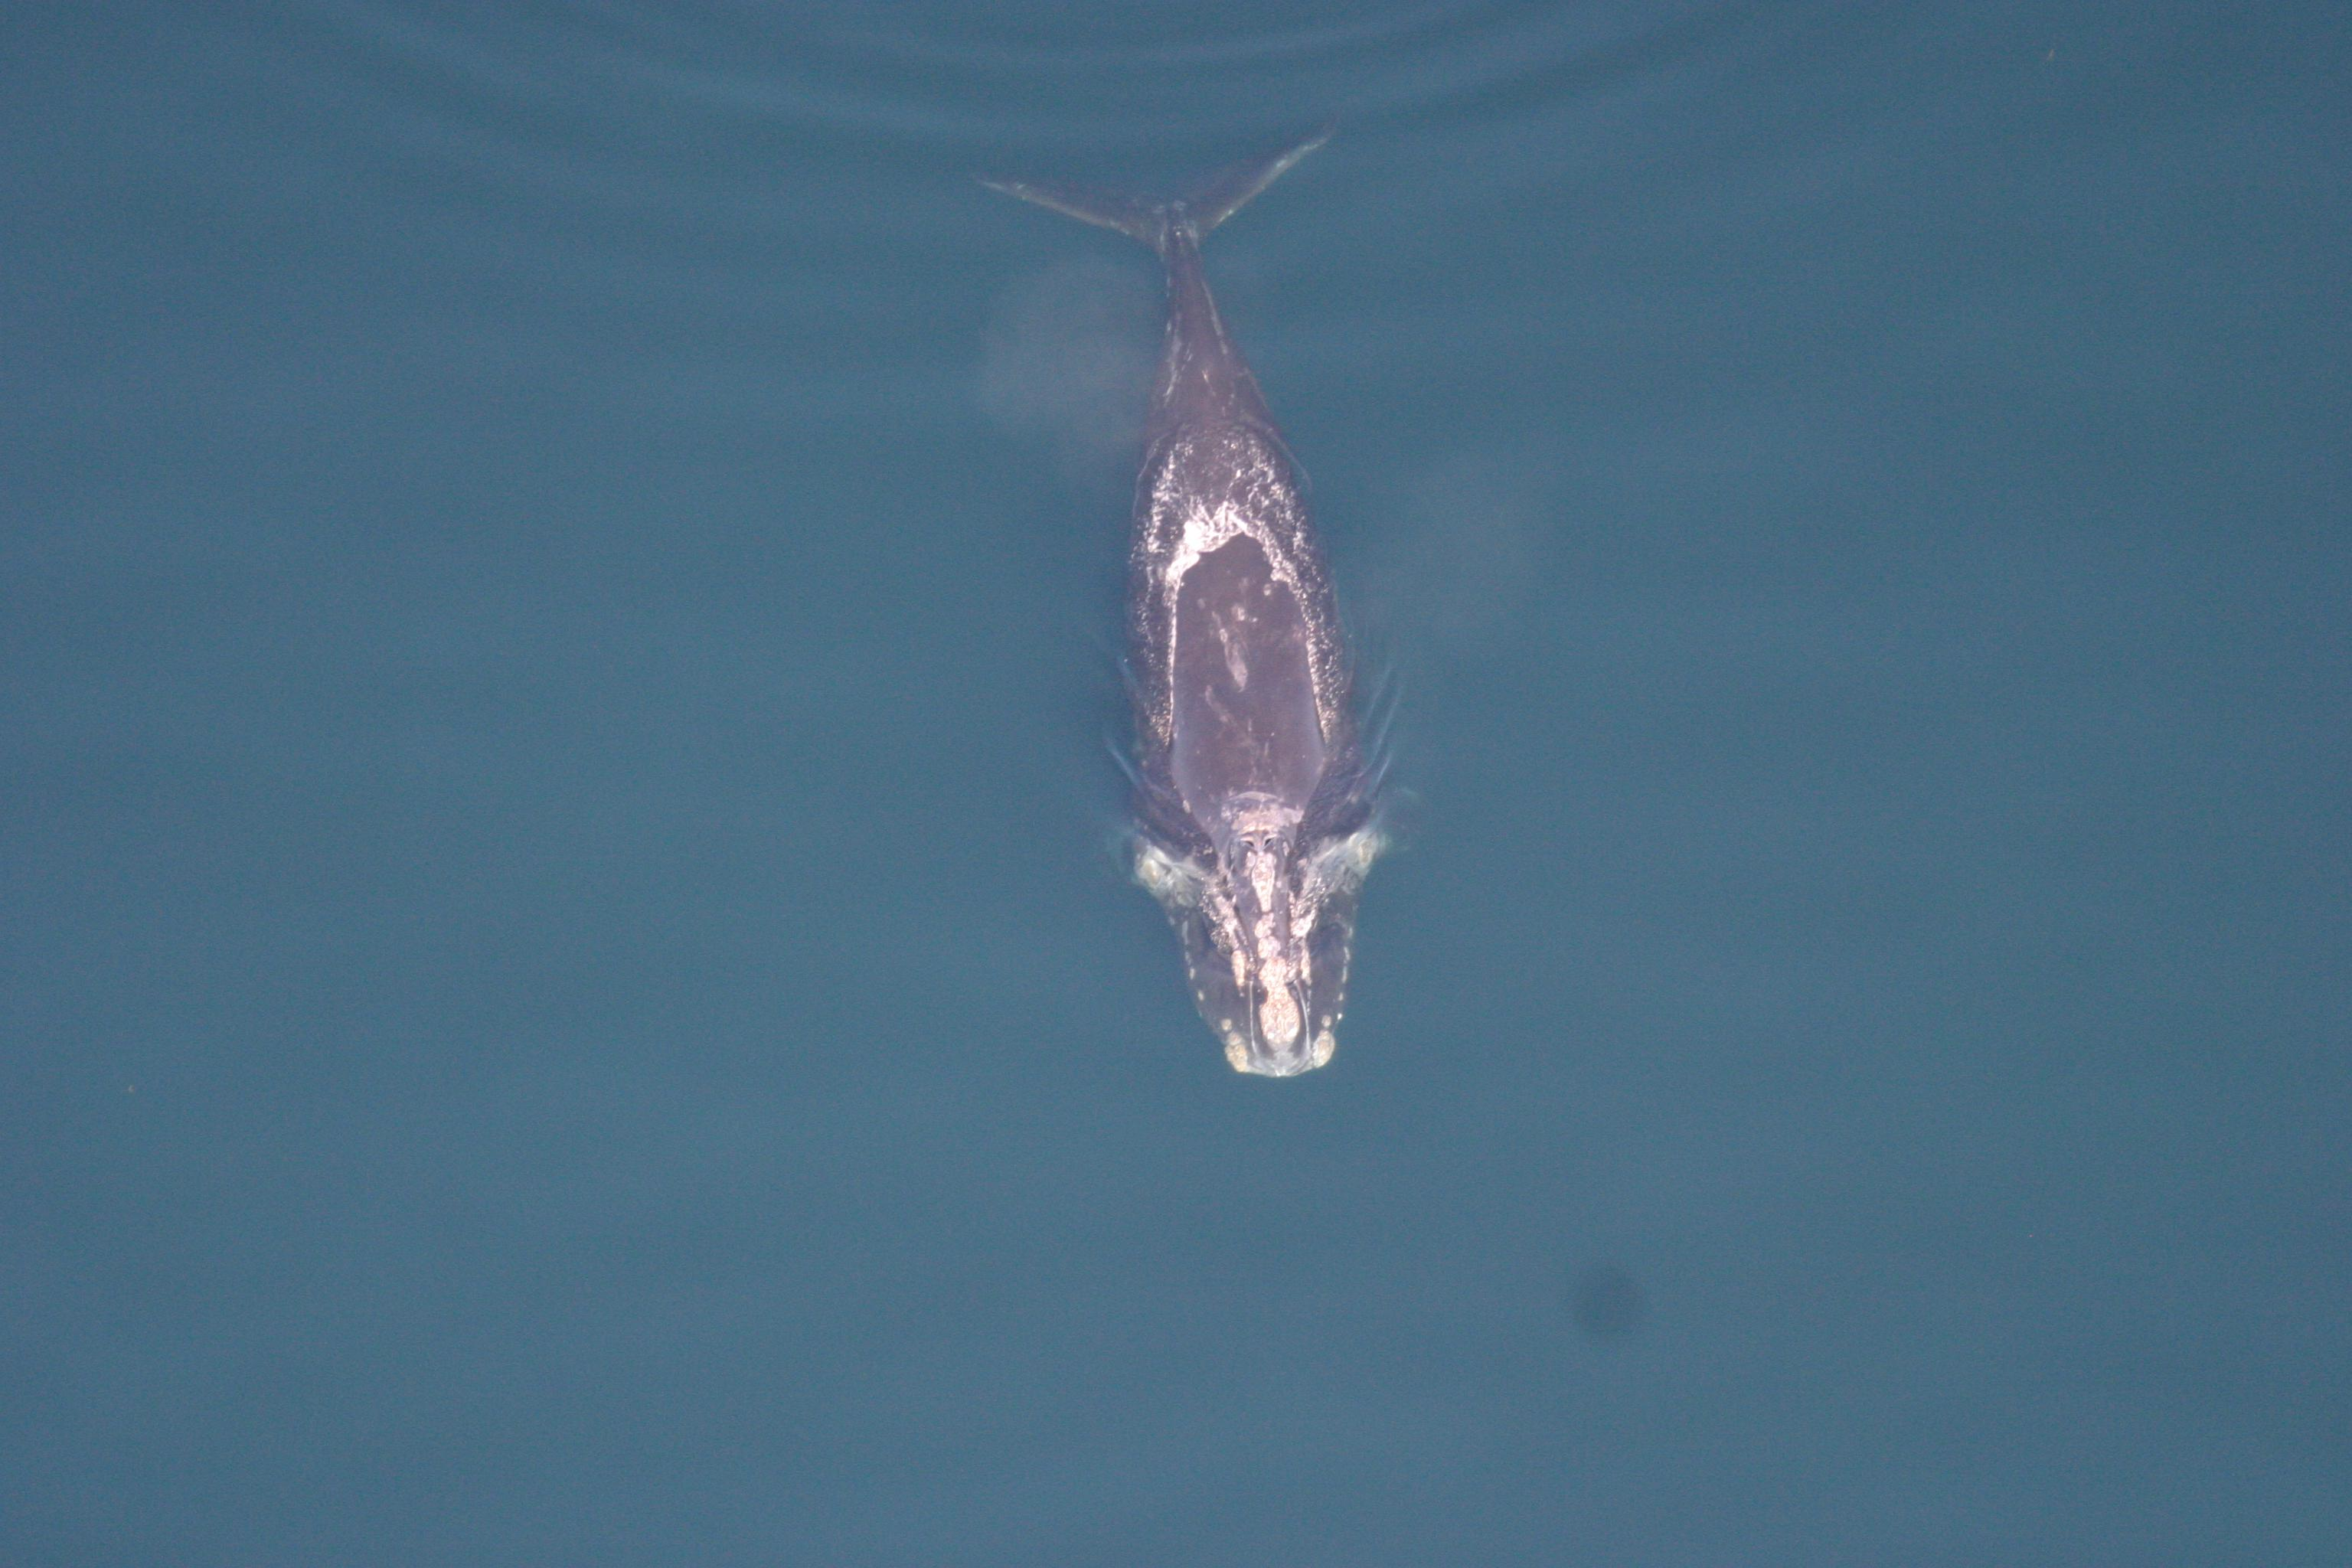
\includegraphics[scale=.08]{example.png}
\caption{Example from data set.}
\end{figure}
\end{frame}

\begin{frame}{Data Example}
\begin{figure}
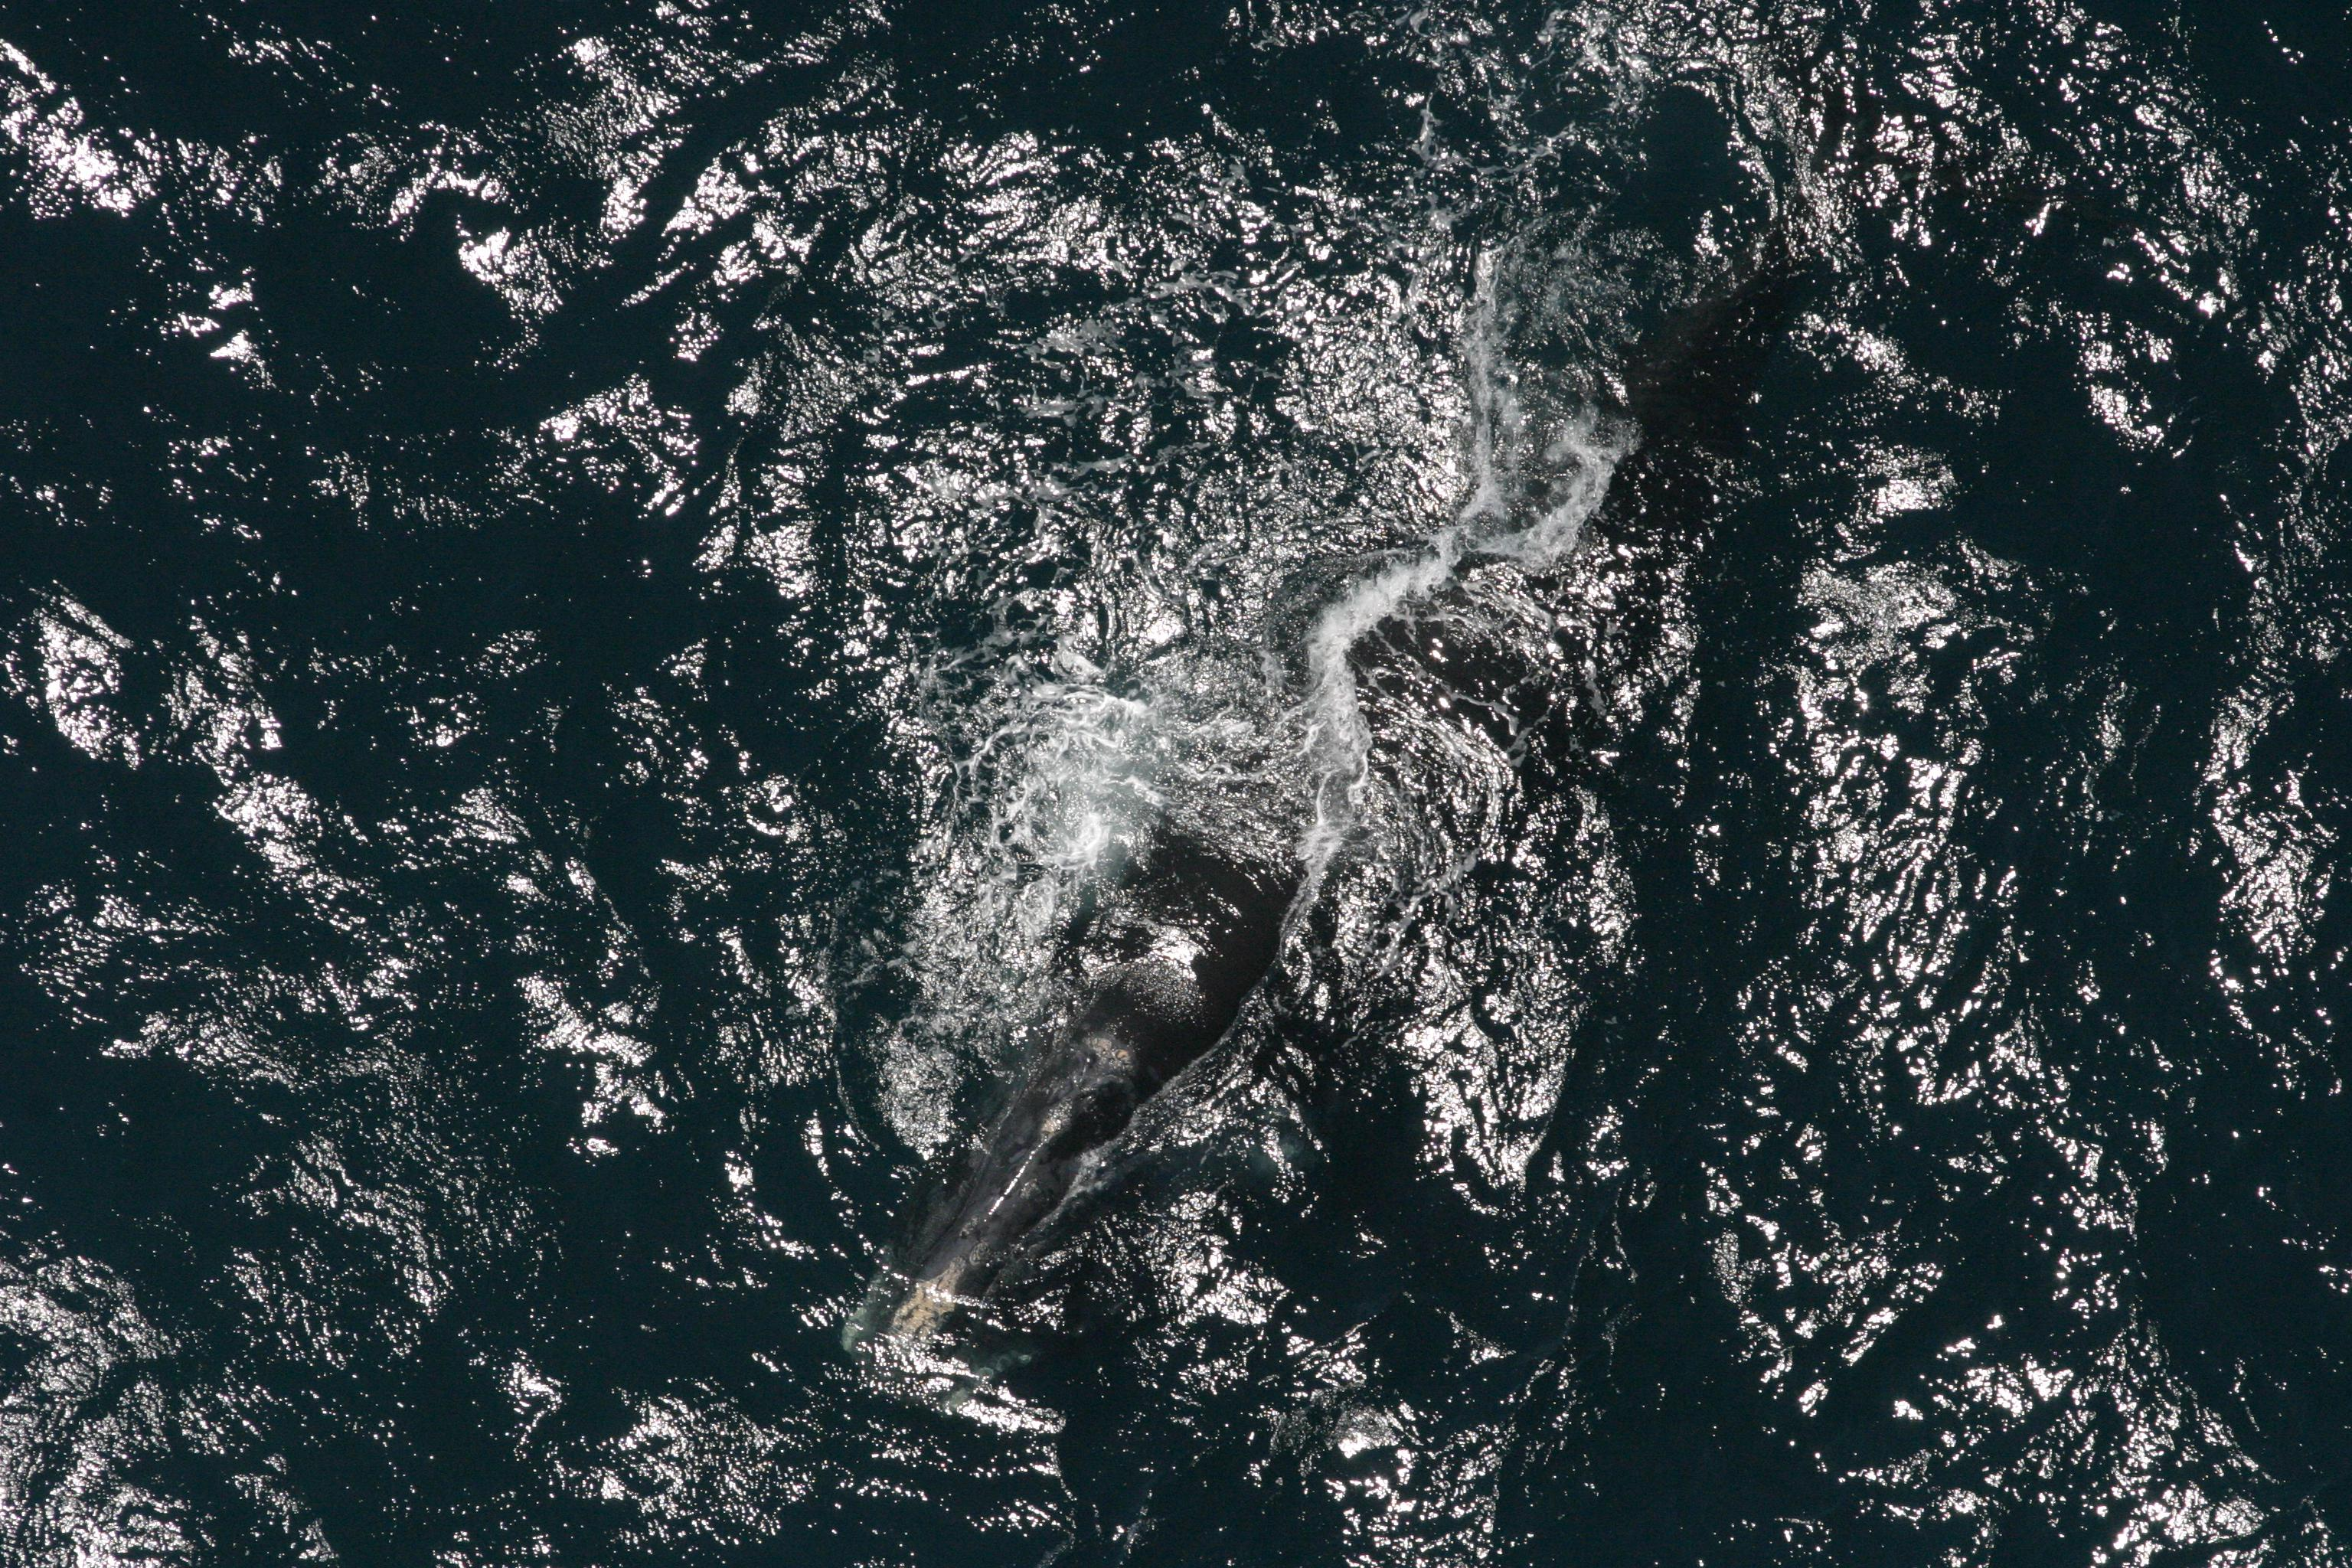
\includegraphics[scale=.08]{example2.png}
\caption{Different lighting and angle.}
\end{figure}
\end{frame}

\begin{frame}{Noise in Data}
\begin{itemize}
\item Other whales
\item Dolphins
\item Birds
\item Surface reflectivity
\item Dirty/clouded water
\end{itemize}
\end{frame}

\begin{frame}{Training Data}
\begin{itemize}
\item List of photos with whale ID provided
\item Label whales by hand to teach recognizer.
\end{itemize}
\begin{figure}
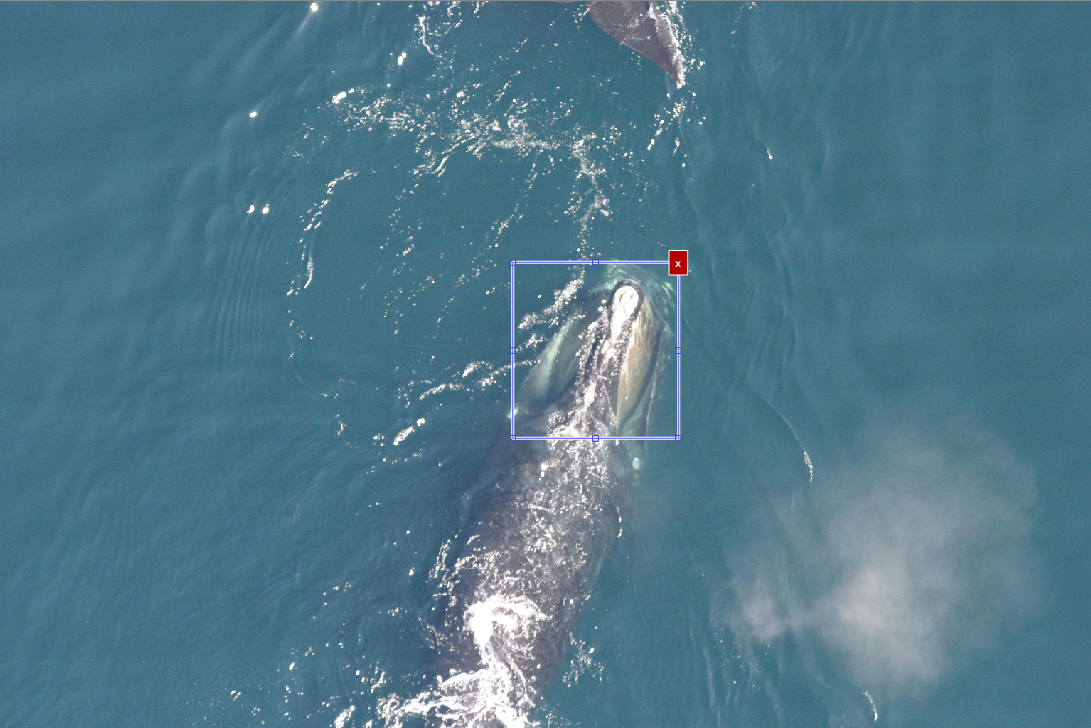
\includegraphics[scale=.25]{label.png}
\end{figure}
\end{frame}

\begin{frame}{Matlab Cascade Object Detector}
\begin{itemize}
\item Machine learning tool
\item Trains in stages
\item Requires positive and negative examples
\item Alternatives: opencv haarcascade, edge detection
\end{itemize}
\end{frame}

\begin{frame}{Matlab Cascade Object Detector}
Parameters:
\begin{itemize}
\item Number of Training stages: 7-11
\item False Alarm Rate: .01
\end{itemize}
\end{frame}

\begin{frame}{Results}
\begin{figure}
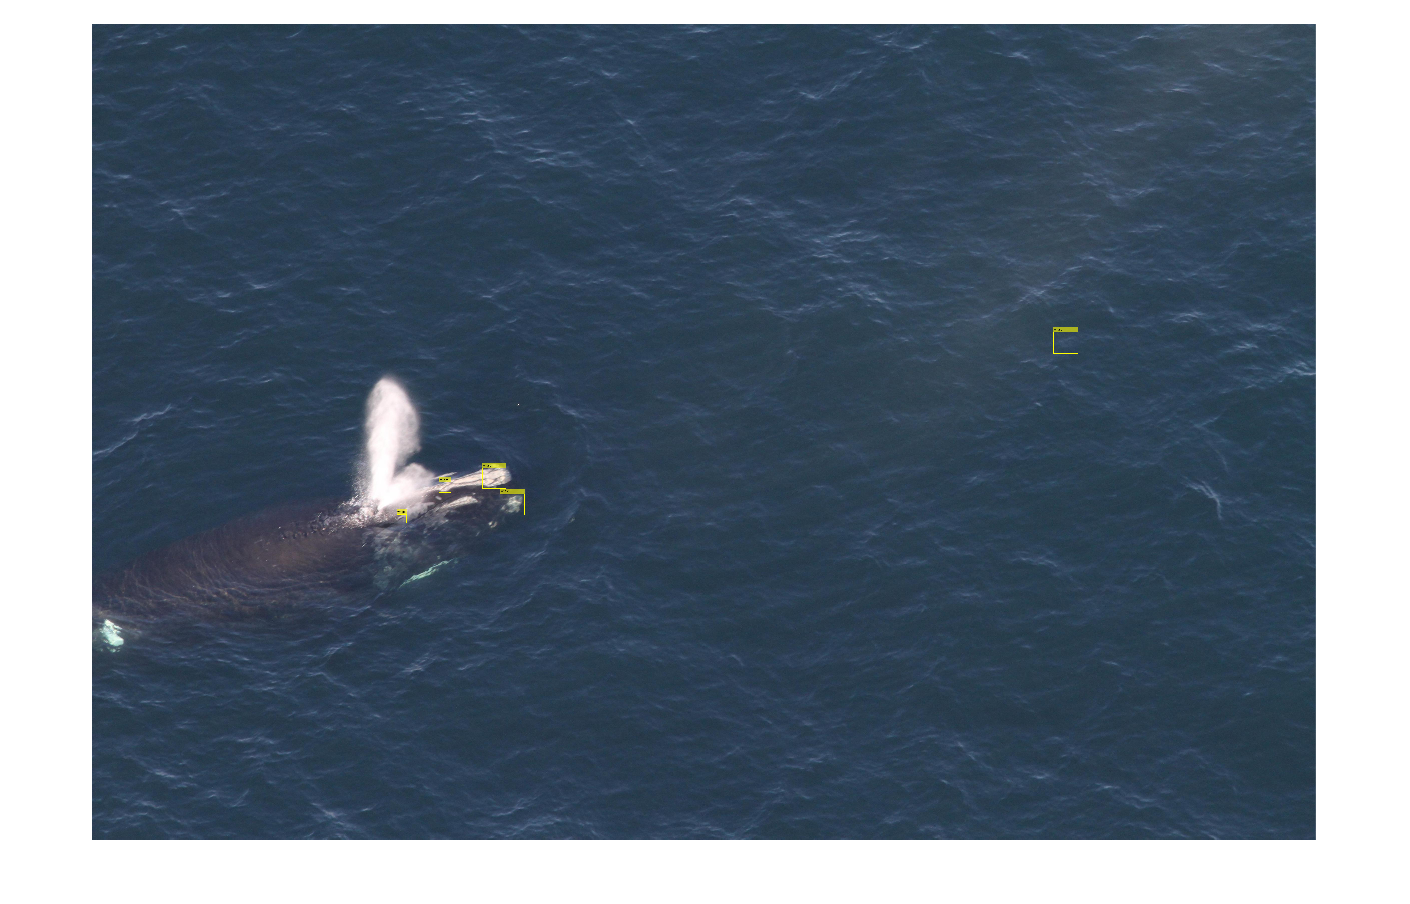
\includegraphics[scale=.23]{recog.png}
\caption{Worst case example. Boxes are "detected whales."}
\end{figure}
\end{frame}

\section{Identification}
\begin{frame}{Approaches}
\begin{itemize}
\item Neural Network
\item Deep-Belief Network
\end{itemize}
\end{frame}

\subsection{Neural Network}
\begin{frame}{Choice: Neural Network}
\begin{itemize}
\item Can handle image input
\item Capable of classifying image to distinct outputs
\item Could potentially be parallelized
\end{itemize}
\end{frame}

\begin{frame}{Design Decisions}
\begin{itemize}
\item Written in Java
\item Input is pixels from 32x30 greyscale images
\item Each pixel is one input
\item Each layer is fully connected
\end{itemize}
\end{frame}

\begin{frame}{Design Decisions}
\begin{itemize}
\item Feed forward network
\item Backpropogation for learning
\item Multiple training epochs required
\end{itemize}
\end{frame}

\begin{frame}{Visualization}
\begin{figure}
\includegraphics[scale=.4]{ann.png}
\end{figure}
\end{frame}

\begin{frame}{Results/Issues}
\begin{itemize}
\item Training requires large amount of time (hours-days)
\item Full output set requires large amount of time
\item Current Issue: input inconsistency from matlab
\end{itemize}
\end{frame}

\subsection{Deep Belief Network}
\begin{frame}{Choice: Deep Belief Network}
\begin{itemize}
\item Deep learning is new/popular
\item Can understand image input
\item Java library available
\item Alternative: SVM
\end{itemize}
\end{frame}

\begin{frame}{Deep Learning 4 Java}
\begin{itemize}
\item Framework for deep learning
\item Can be used with Hadoop or GPUs (fast)
\item Has data input/output system (Canova)
\end{itemize}
\end{frame}

\begin{frame}{DL4J Statistics}
\begin{figure}
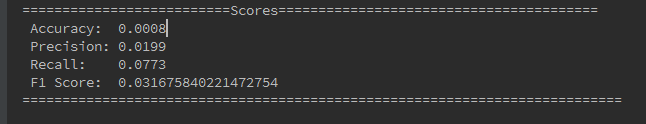
\includegraphics[scale=1]{stats.png}
\caption{Statistical sample output from test program}
\end{figure}
\end{frame}


\begin{frame}{Results/Issues}
\begin{itemize}
\item DL4J has lots of examples, but bad documentation
\item Belief network engine currently misinterprets input, does not currently
produce output
\end{itemize}
\end{frame}

\section{Conclusion}
\begin{frame}{Summary}
So far we've discussed:
\begin{itemize}
\item Whale detection with matlab
\item Whale identification with neural network
\item Whale identification with deep belief network
\end{itemize}
\end{frame}

\begin{frame}{Continuing Work}
\begin{itemize}
\item Find solution for multiple whales recognized
\item Identify training issue in DL4J
\item Transfer neural network to batch learning and use MPI/Palmetto?
\end{itemize}
\end{frame}

\begin{frame}{References}
\bibliography{project.bib}
\nocite{*}
\end{frame}

\end{document}
